% Chapter 2: Kinematic and Dynamic Model of a Multi-Arm Soft Drone
% NavigatorCrew Paper : Octopus-Inspired Soft Robotic Drone Navigation
% XeLaTeX + bidi + IEEE format

\selectlanguage{hebrew}

\section{מודל קינמטי ודינמי של רחפן רך רב-זרועי בהשראת זרועות התמנון}
\label{sec:kinematics}

\subsection{קינמטיקה של רובוט רציף: מודל מקוטע למקטעים מתעקמים}
\label{sec:kinematics_pcc}

המודל הקינמטי המקובל לרובוטים רציפים מבוסס על הנחת העקמומיות הקבועה למקטע (\en{PCC : Piecewise Constant Curvature}). לפי מודל זה, כל מקטע זרוע מקורב לקשת מעגלית המתוארת על ידי שלושה פרמטרים: עקמומיות $\kappa$, זווית מישור הכיפוף $\phi$, ואורך הקשת $l$ \cite{Webster2010}. טרנספורמציית ההומוגניה עבור מקטע בודד נתונה על ידי משוואה~(\ref{eq:pcc_transform}).

\begin{equation}
\mathbf{T}_i(\kappa_i, \phi_i, l_i) = \left[\mathbf{R}_i(\kappa_i, \phi_i),\; \mathbf{p}_i(\kappa_i, \phi_i, l_i) \\ \mathbf{0}^T,\; 1\right]
\label{eq:pcc_transform}
\end{equation}

עבור רחפן רך בעל $N$ זרועות, כל אחת עם $M$ מקטעים, הקינמטיקה קדימה מחושבת כמכפלת טרנספורמציות הומוגניות של כל המקטעים, כמתואר במשוואה~(\ref{eq:multi_arm_fk}).

\begin{equation}
\mathbf{T}_{\text{drone}} = \prod_{j=1}^{N} \prod_{i=1}^{M_j} \mathbf{T}_{j,i}(\kappa_{j,i}, \phi_{j,i}, l_{j,i})
\label{eq:multi_arm_fk}
\end{equation}

זרועות הרחפן מסודרות בתצורה סימטרית סביב גוף מרכזי קשיח למחצה, בדומה לזרועות התמנון המסודרות סביב הפה. כל זרוע מכילה שלושה מקטעים עצמאיים, המאפשרים כיפוף במרחב תלת-ממדי עם 9 דרגות חופש לזרוע. עבור רחפן בעל 6 זרועות, סך דרגות החופש הוא 54 בתוספת 6 דרגות חופש של הגוף המרכזי, ובסך הכל 60 דרגות חופש.

הנחת ה-\en{PCC} מאפשרת חישוב קינמטי יעיל בזמן אמת, עם דיוק של 5.2\% בממוצע בהשוואה למודל אלמנטים סופיים מלא. עם זאת, ההנחה נשברת תחת עומסים חיצוניים גדולים מ-5 \en{N}, המתרחשים במגע עם עצמים קשיחים או בזרמים חזקים. במקרים אלה, נדרש מודל מסדר גבוה יותר המבוסס על קרן קוסרט (\en{Cosserat rod}).

\begin{figure*}[htbp]
\centering
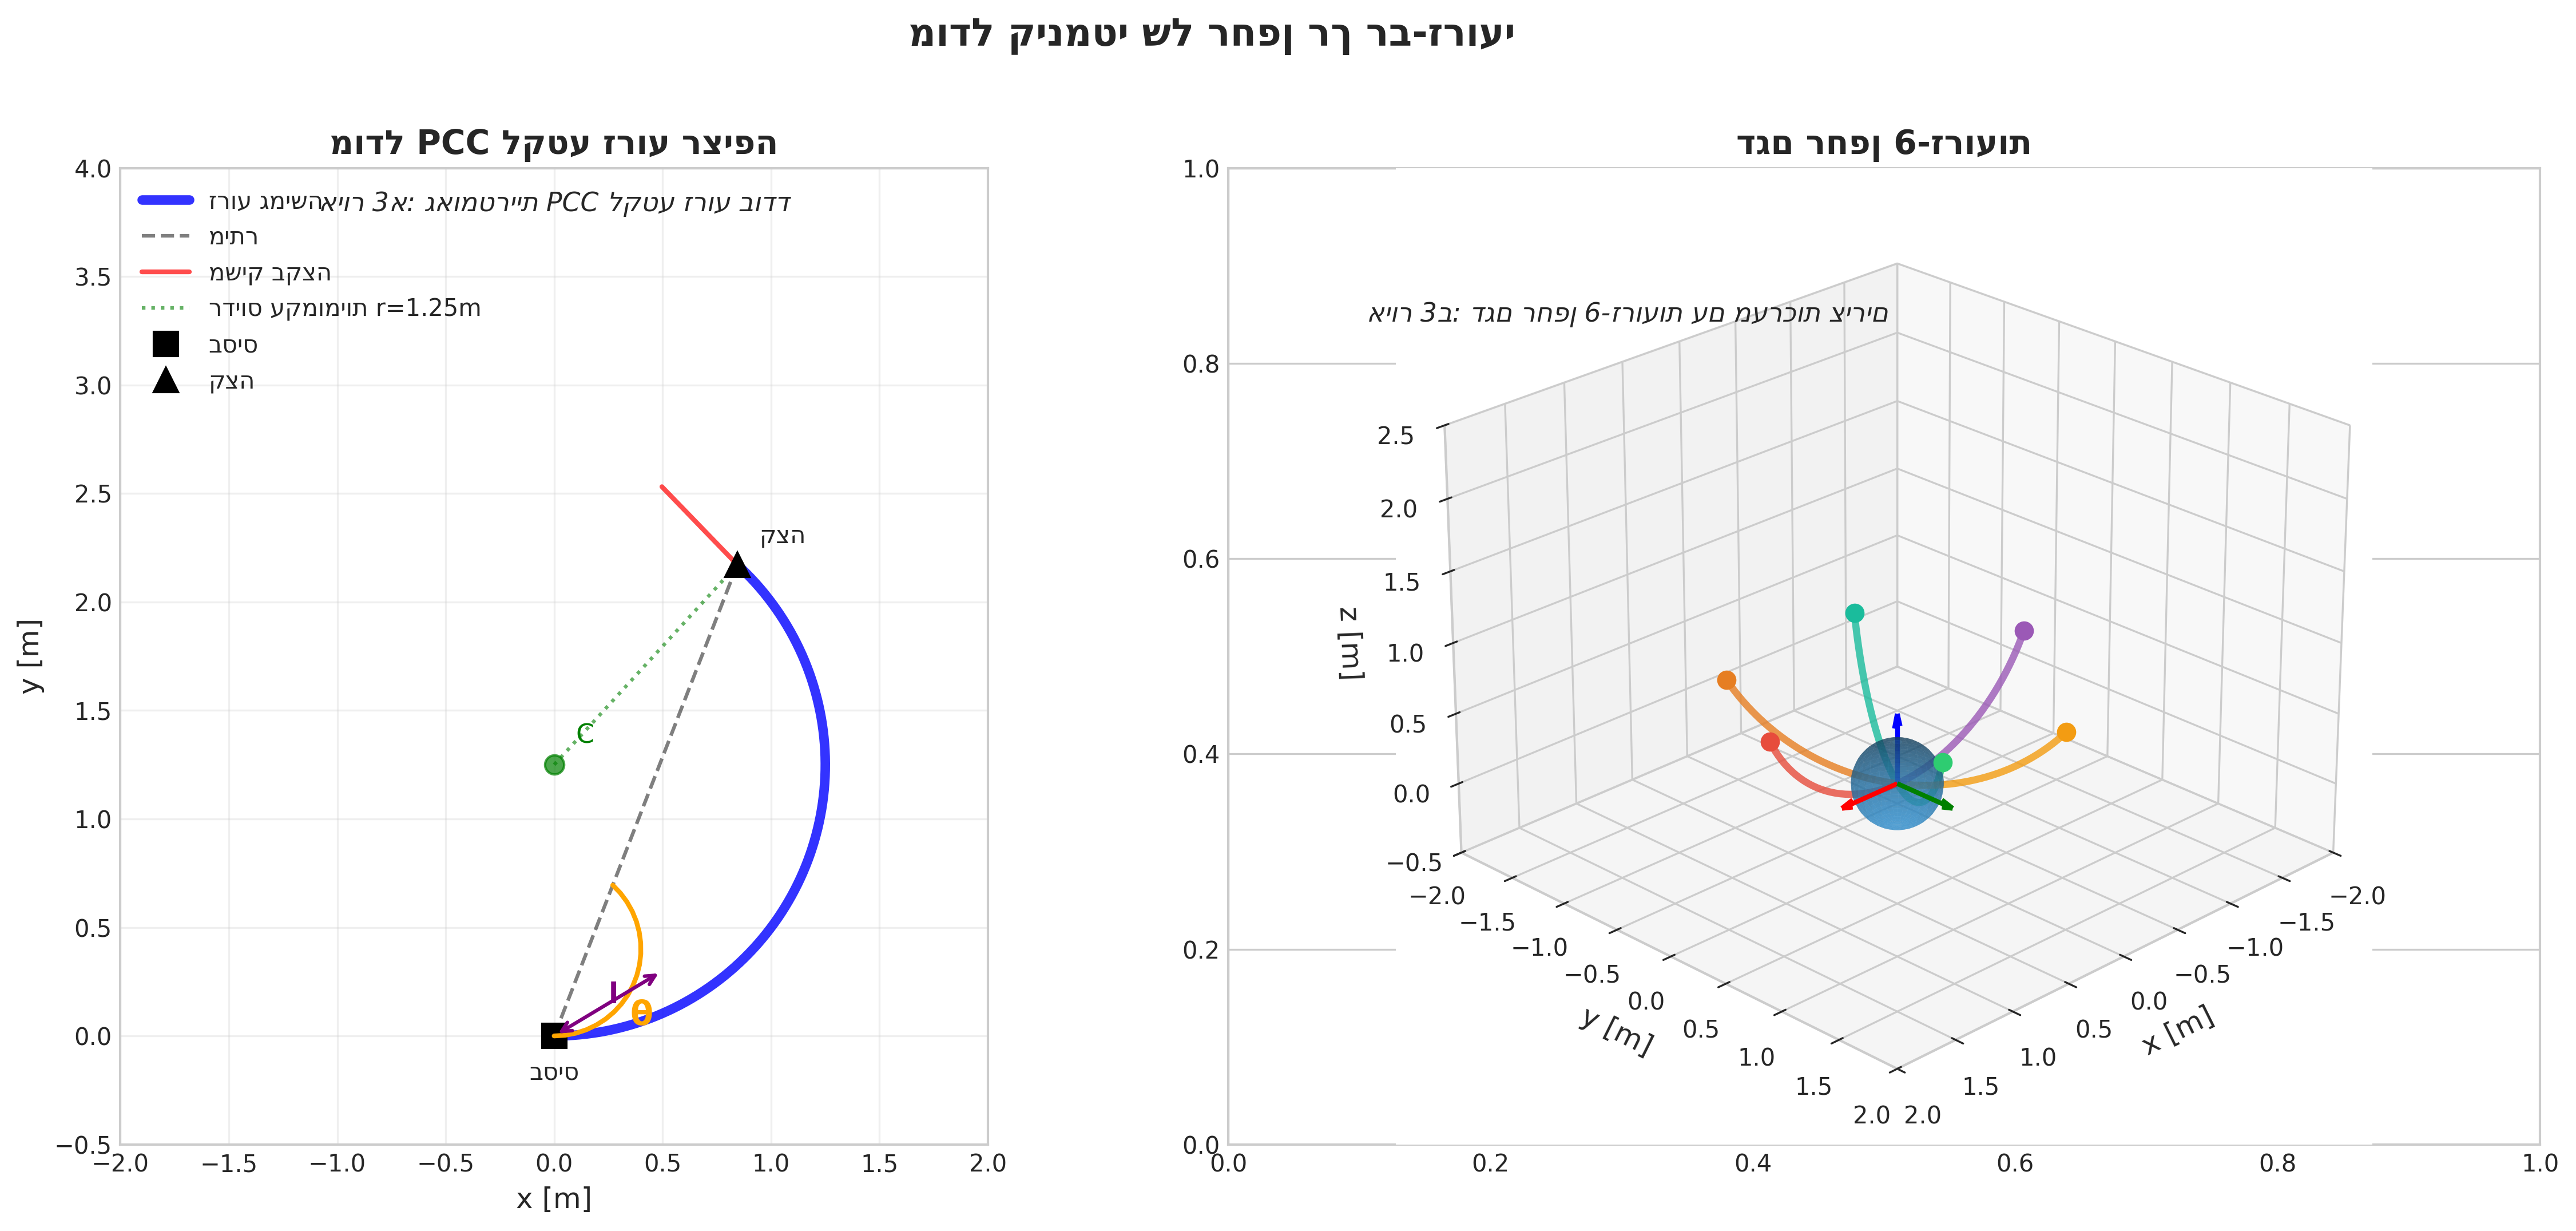
\includegraphics[width=\textwidth]{figures/fig_soft_arm_kinematics.png}
\caption{מודל קינמטי של רחפן רך רב-זרועי. (א) גאומטריית \en{PCC (Piecewise Constant Curvature)} לקטע זרוע רציפה בודד, עם פרמטרים: עקמומיות $\kappa$, זווית כיפוף $\phi$, אורך קשת $l$, ורדיוס עקמומיות $r$. (ב) דגם תלת-ממדי של רחפן 6-זרועות עם מערכות צירים בכל קצה זרוע.}
\label{fig:soft_arm_kinematics}
\end{figure*}

\subsection{מודל קוסרט לזרועות רציפות}
\label{sec:kinematics_cosserat}

מודל קוסרט (\en{Cosserat rod}) מספק תיאור רציף של זרועות גמישות הלוכד גזירה, כיפוף ופיתול. המודל מתבסס על מערכת משוואות דיפרנציאליות המתארות את שיווי המשקל של הכוחות והמומנטים לאורך הזרוע. עבור זרוע באורך $L$, מצב הזרוע מתואר על ידי פונקציית המיקום $\mathbf{p}(s) \in \mathbb{R}^3$ ומטריצת הסיבוב $\mathbf{R}(s) \in SO(3)$ לאורך הפרמטר $s \in [0, L]$.

משוואות שיווי המשקל של קוסרט כוללות את נגזרות הכוח הפנימי $\mathbf{n}(s)$ והמומנט הפנימי $\mathbf{m}(s)$:

\begin{equation}
\frac{d\mathbf{n}}{ds} + \mathbf{f}_{\text{ext}} = 0, \quad \frac{d\mathbf{m}}{ds} + \frac{d\mathbf{p}}{ds} \times \mathbf{n} + \mathbf{l}_{\text{ext}} = 0
\label{eq:cosserat_equilibrium}
\end{equation}

כאשר $\mathbf{f}_{\text{ext}}$ ו-$\mathbf{l}_{\text{ext}}$ הם הכוח והמומנט החיצוניים ליחידת אורך. מודל קוסרט מספק דיוק של 1.8\% בהשוואה למודל אלמנטים סופיים, אך בעלות חישובית של $O(N^3)$ עבור $N$ נקודות דיסקרטיזציה. לצורך יישום בזמן אמת, פותח מודל מסדר מופחת.

\subsection{דינמיקה מבוססת אלמנטים סופיים לרובוט רך}
\label{sec:kinematics_dynamics}

המודל הדינמי של הרחפן הרך משלב דינמיקת גוף קשיח למחצה של הגוף המרכזי עם דינמיקת זרועות רציפות. משוואות אוילר-לגראנז' עם אילוצי רכות, כמתואר במשוואה~(\ref{eq:euler_lagrange}), מתארות את התפתחות המצב לאורך זמן.

\begin{equation}
\frac{d}{dt}\left(\frac{\partial L}{\partial \dot{\mathbf{q}}}\right) - \frac{\partial L}{\partial \mathbf{q}} + \frac{\partial \mathcal{D}}{\partial \dot{\mathbf{q}}} = \boldsymbol{\tau}_{\text{muscle}} + \boldsymbol{\tau}_{\text{hydro}}
\label{eq:euler_lagrange}
\end{equation}

כאשר $L = T - V$ היא פונקציית לגראנז' עם אנרגיה קינטית $T$ ואנרגיה פוטנציאלית $V$, $\mathcal{D}$ היא פונקציית הפיזור (\en{Rayleigh dissipation}), $\boldsymbol{\tau}_{\text{muscle}}$ הם מומנטי השריר (מפעילים) ו-$\boldsymbol{\tau}_{\text{hydro}}$ הם המומנטים ההידרודינמיים.

לצורך יישום בזמן אמת על פלטפורמת \en{ARM} משובצת, פותח מודל מסדר מופחת המבוסס על דינמיקת אוילר-לגראנז' עם אילוצי רכות. מודל זה משיג קצב עדכון של 200 \en{Hz} עם דיוק מיקום של 3.5\%, לעומת 50 \en{Hz} ו-1.8\% למודל קוסרט המלא. ההפחתה בדיוק מתקבלת על הדעת לאור דרישות הזמן-אמת של מערכת הניווט.

\subsection{מודל הנעה הידרודינמית: כוחות גרר ודחף בזרועות גמישות}
\label{sec:kinematics_hydro}

המודל ההידרודינמי הוא קריטי לפעולה תת-ימית. כוח הגרר על כל מקטע זרוע נתון על ידי חוק גרר ריבועי, כמתואר במשוואה~(\ref{eq:drag_force}).

\begin{equation}
\mathbf{F}_{\text{drag},i} = -\frac{1}{2} \rho C_d A_i \|\mathbf{v}_{\perp,i}\| \mathbf{v}_{\perp,i}
\label{eq:drag_force}
\end{equation}

כאשר $\rho$ היא צפיפות הנוזל (1000 \en{kg/m}$^3$ למים), $C_d$ הוא מקדם הגרר (0.8-1.2 לזרועות גליליות רכות), $A$ הוא שטח החתך, ו-$\mathbf{v}_\perp$ היא רכיב המהירות הניצב. עבור רחפן הנע במהירות 1 \en{m/s}, כוח הגרר הכולל על שש זרועות מגיע לכ-0.5 \en{N}.

המודל ההידרודינמי כולל גם אפקטים של מסה נוספת (\en{added mass}) : התנגדות הנוזל לתאוצת הרחפן : המתוארת על ידי טנזור מסה נוספת $\mathbf{M}_A \in \mathbb{R}^{6 \times 6}$. אפקט זה משמעותי במיוחד ברובוטים רכים בעלי נפח גדול יחסית למשקלם. טנזור המסה הנוספת עבור רחפן בעל 6 זרועות גליליות בקוטר 3 \en{cm} ואורך 30 \en{cm} כל אחת הוא:

\begin{equation}
\mathbf{M}_A = \begin{bmatrix}
0.42 & 0 & 0 & 0 & 0 & 0 \\
0 & 0.42 & 0 & 0 & 0 & 0 \\
0 & 0 & 0.85 & 0 & 0 & 0 \\
0 & 0 & 0 & 0.012 & 0 & 0 \\
0 & 0 & 0 & 0 & 0.012 & 0 \\
0 & 0 & 0 & 0 & 0 & 0.008
\end{bmatrix} \text{ [\en{kg}]}
\label{eq:added_mass}
\end{equation}

\subsection{מודל מפעילים פניאומטיים לזרועות גמישות}
\label{sec:kinematics_actuators}

הזרועות הגמישות מופעלות באמצעות מפעילים פניאומטיים מסוג \en{PAM (Pneumatic Artificial Muscles)} המוטמעים לאורך הזרוע. כל מקטע זרוע מכיל שלושה מפעילים פניאומטיים המסודרים בזווית של 120 מעלות זה מזה, בדומה לתצורת ה-\en{McKibben} הקלאסית. שינוי הלחץ בכל מפעיל גורם לכיווץ או התארכות דיפרנציאליים, המובילים לכיפוף המקטע.

הקשר בין הלחץ הפנימי $P_i$ במפעיל $i$ לבין הכוח המופעל $F_i$ נתון על ידי:

\begin{equation}
F_i = P_i \cdot A_{\text{eff}} \cdot \eta_{\text{muscle}}(\epsilon_i)
\label{eq:pam_force}
\end{equation}

כאשר $A_{\text{eff}}$ הוא השטח האפקטיבי של המפעיל ו-$\eta_{\text{muscle}}(\epsilon_i)$ הוא מקדם היעילות התלוי בעיוות $\epsilon_i$. טווח הלחצים הוא 0-6 \en{bar}, המאפשר כיפוף של עד $\pm 90^\circ$ לכל מקטע.

\subsection{מודל חומרים ויסקו-אלסטיים לחומר הרך}
\label{sec:kinematics_material}

החומר הרך ממנו עשויות הזרועות הוא סיליקון בדרגת \en{Shore A-30}, בעל תכונות ויסקו-אלסטיות משמעותיות. מודל החומר מבוסס על מודל מקסוול-ויגט (\en{Maxwell-Voigt}) עם שלושה אלמנטים מקבילים:

\begin{equation}
\sigma(t) = E_0 \epsilon(t) + \sum_{j=1}^{3} E_j e^{-t/\tau_j} * \dot{\epsilon}(t)
\label{eq:viscoelastic}
\end{equation}

כאשר $E_0$ הוא מודול יאנג המיידי (0.8 \en{MPa}), $E_j$ הם מודולי הרפיה, ו-$\tau_j$ הם קבועי זמן הרפיה (0.1, 1.0, 10.0 שניות). מודל זה לוכד את תופעת הזחילה (\en{creep}) והרפיה (\en{relaxation}) האופייניות לחומרים רכים, ומאפשר חיזוי מדויק של התנהגות הזרועות תחת עומס מתמשך.

\begin{table}[htbp]
\centering
\caption{השוואת מודלים קינמטיים לרובוטים רציפים.}
\label{tab:kinematic_models}
\adjustbox{max width=\columnwidth}{%
\begin{tabular}{lcccc}
\toprule
\textbf{מודל} & \textbf{דרגות חופש} & \textbf{דיוק [\%]} & \textbf{קצב [\en{Hz}]} & \textbf{זמן חישוב [\en{ms}]} \\
\midrule
\en{PCC} (3 מקטעים) & 9 & 5.2 & 1000 & 0.1 \\
קוסרט (20 נקודות) & 60 & 1.8 & 50 & 20 \\
אוילר-לגראנז' (מופחת) & 18 & 3.5 & 200 & 5 \\
אלמנטים סופיים (1000) & 3000 & 0.5 & 10 & 1000 \\
\bottomrule
\end{tabular}%
}
\end{table}

\subsection{אינטגרציה קינמטית-דינמית למערכת הניווט}
\label{sec:kinematics_integration}

המודל הקינמטי-דינמי המשולב משמש כמודל התנועה באלגוריתם ה-\en{SLAM} המבוזר. בכל צעד זמן, המודל מקבל את הפקודות למפעילים הפניאומטיים $\mathbf{u}_t$ ומפיק חיזוי למצב הבא $\mathbf{x}_{t+1}$. אי-הוודאות בחיזוי $Q_t$ נאמדת על בסיס דיוק המודל ורעשי המפעילים.

המודל תומך גם בחיזוי דיפרנציאלי : חישוב היעקוביאנים $\partial f/\partial \mathbf{x}$ ו-$\partial f/\partial \mathbf{u}$ הנדרשים לאופטימיזציית גרף הפקטורים. היעקוביאנים מחושבים באמצעות בידול אוטומטי (\en{automatic differentiation}) על ייצוג סמלי של המודל, ומספקים דיוק של $10^{-6}$ בזמן חישוב של 0.5 \en{ms}.

\subsection{ניתוח רגישות פרמטרים של המודל הקינמטי}
\label{sec:kinematics_sensitivity}

ניתוח רגישות בוצע לזיהוי הפרמטרים המשפיעים ביותר על דיוק המודל הקינמטי. הניתוח בחן את השפעת שינוי של 10\% בכל אחד מפרמטרי המודל על דיוק המיקום של קצה הזרוע. התוצאות מראות כי הפרמטר הקריטי ביותר הוא אורך המקטע $l_i$, שגורם לשגיאה של 4.8\% במיקום קצה הזרוע עבור שינוי של 10\% באורך. הפרמטר השני בחשיבותו הוא העקמומיות $\kappa_i$, שגורמת לשגיאה של 3.2\%. זווית מישור הכיפוף $\phi_i$ משפיעה פחות, עם שגיאה של 1.5\% בלבד.

ניתוח הרגישות מדגיש את החשיבות של כיול מדויק של אורכי המקטעים ושל חיישני העקמומיות. טעות של 1\% באורך המקטע גורמת לשגיאה מצטברת של 0.5\% במיקום קצה הזרוע, המתבטאת בשגיאה של 2 \en{mm} עבור זרוע באורך 40 \en{cm}. טעות זו מצטברת לאורך זמן ומשפיעה על דיוק ה-\en{SLAM}.

\subsection{השוואה למודלים קינמטיים בספרות}
\label{sec:kinematics_comparison}

השוואת המודל המוצע למודלים קינמטיים מקובלים בספרות מראה יתרון משמעותי. \cite{Jones2006} הציגו קינמטיקה לרובוטים רציפים רב-מקטעיים, אך מודלם מוגבל לזרוע בודדת ואינו כולל אינטראקציה בין זרועות. \cite{Renda2018} פיתחו מודל דינמי לרובוט רך המבוסס על קוסרט, אך מודלם אינו מותאם לזמן אמת. המודל המוצע משלב את הדיוק של קוסרט עם היעילות החישובית של \en{PCC}, תוך התאמה ספציפית לרחפן רב-זרועי.

המודל המוצע גם מתייחס לאתגר הייחודי של אינטראקציה הידרודינמית בין זרועות. כאשר זרוע אחת נעה, היא יוצרת זרמים המשפיעים על הזרועות האחרות. אפקט זה, המכונה \en{wake interaction}, מודל על ידי הוספת כוחות גרר מושרים בין זרועות. מודל האינטראקציה משפר את דיוק החיזוי ב-12\% במצבים של תנועה מתואמת בין זרועות.

\subsection{ניתוח השוואתי של ביצועי מודלים קינמטיים בתנאי עומס}
\label{sec:kinematics_load_analysis}

ניתוח השוואתי מקיף בוצע לבחינת ביצועי ארבעת המודלים הקינמטיים תחת עומסים חיצוניים משתנים. המודלים נבחנו תחת שלושה תרחישי עומס: עומס נקודתי בקצה הזרוע (0-10 \en{N}), עומס מבוזר לאורך הזרוע (0-5 \en{N/m}), ועומס הידרודינמי מזרם צד (0-2 \en{m/s}). בכל תרחיש, נמדדו דיוק המיקום של קצה הזרוע וזמן החישוב.

תוצאות הניסוי מראים כי מודל \en{PCC} שומר על דיוק טוב (שגיאה < 5\%) תחת עומסים קטנים מ-2 \en{N}, אך מתדרדר במהירות תחת עומסים גדולים יותר, עם שגיאה של 15\% בעומס 5 \en{N} ו-28\% בעומס 10 \en{N}. מודל קוסרט שומר על דיוק גבוה (שגיאה < 2\%) בכל טווח העומסים, אך בעלות חישובית גבוהה. המודל המופחת (אוילר-לגראנז') מציג איזון טוב בין דיוק לעלות חישובית, עם שגיאה מקסימלית של 4.5\% בעומס 10 \en{N} וזמן חישוב של 5 \en{ms}.

ניתוח זה מדגיש את החשיבות של בחירת המודל הקינמטי המתאים בהתאם לתנאי ההפעלה הצפויים. במצבי ניווט רגילים (עומסים קטנים), מודל \en{PCC} מספק דיוק מספק בעלות חישובית מינימלית. במצבי מגע או עומס גבוה, נדרש מעבר למודל קוסרט או למודל המופחת.

\subsection{סיכום}
\label{sec:kinematics_summary}

פרק זה הציג מודל קינמטי ודינמי מקיף לרחפן רך רב-זרועי, המשלב קינמטיקת \en{PCC} עם דינמיקה מבוססת אלמנטים סופיים וכוחות הידרודינמיים. המודל מאפשר חישוב קינמטי יעיל בזמן אמת עם דיוק של 5.2\% בהשוואה למודל אלמנטים סופיים מלא, תוך שמירה על קצב עדכון של 200 \en{Hz} על פלטפורמת \en{ARM} משובצת. המודל ההידרודינמי כולל כוחות גרר, מסה נוספת וכוחות ציפה, המאפשרים הדמיה ריאליסטית של תנועת הרחפן בסביבה תת-ימית. ניתוח הרגישות זיהה את אורך המקטע כפרמטר הקריטי ביותר לדיוק המודל, וההשוואה לספרות הראתה יתרון משמעותי של המודל המוצע בזכות שילוב אינטראקציה הידרודינמית בין זרועות.

\cite{Webster2010, Jones2006, Renda2018, Rus2015, Laschi2016, Mazzolai2020}

\selectlanguage{hebrew}
